\section{Nao Hardware}
\label{nao:hardware}
Der in dieser Arbeit verwendete Nao ist vom Typ \textit{NAO V3+, V3.2}. Dieser Typ ist 573.2 mm hoch, 290 mm tief und 273.3 mm breit. In Abbildung \myref{f:nao_ov} sind alle Sensoren und Aktoren aufgeführt.
\\
\begin{figure}[H]						
	\centering							
	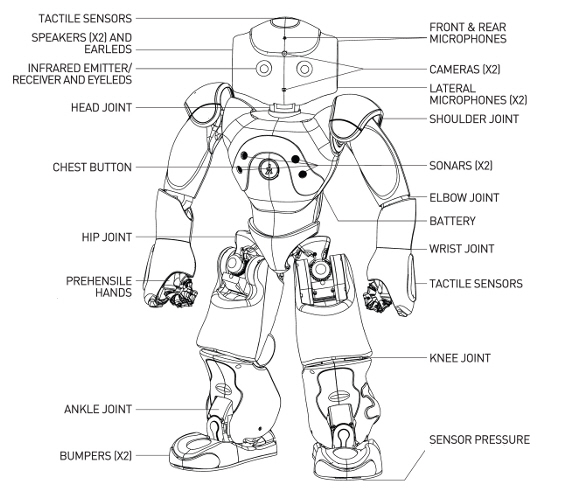
\includegraphics[scale=0.9]{Bilder/nao_overview.jpg}			
	\caption{Übersicht Nao V3.2}						
	\label{f:nao_ov}						
\end{figure}
\noindent
\textbf{Gelenke}
\\
Nao besitzt  im Kopf, den beiden Armen, dem Becken und den beiden Beinen jeweils mehrere Gelenke (\textit{Joints}, siehe Abb. \ref{f:nao_ov}). Damit ist eine umfangreiche Bewegung in alle Richtungen der drei Achsen möglich. Der Kopf lässt sich in Z-Richtung drehen und in Y-Richtung neigen, damit Nao auch räumlich sehen, bzw. Objekte verfolgen kann.
Die Arme weisen die gleichen Gelenke auf, wie ein menschlicher Körper. Dazu gehören Schulter-, Ellenbogen- und Handgelenk. Das Schultergelenk dient dazu, den Arm zu heben/senken und ihn zu öffnen bzw. zu schließen. Das Drehen und Öffnen/Schließen des Unterarms geschieht durch das Ellenbogengelenk in Kombination mit dem Hangelenk. Die Finger der Hand können nur als Ganzes geöffnet bzw. geschlossen werden.
Das Beckengelenk wird dazu benutzt, den Torso von Nao nach vorne oder hinten zu neigen.
Die Beine bestehen aus drei Gelenken: Einem Hüft-, einem Knie- und einem Fußgelenk. Die Bewegungsfreiheit der Beine ähnelt dem des menschlichen Beins, wobei keines der Gelenke in Z-Richtung gedreht werden kann.

Die Bestimmung der Gelenkpositionen erfolgt über einen magnetischen Drehwinkelgeber	mit einer Auflösung von 12 Bit. Das macht beispielsweise bei einem Wert von 4096 pro Umdrehung eine Präzision von 0.1 Grad aus.
\\
\\
\textbf{Gelenkraum Nao}
\\
Da primär die Armbewegungen von Nao nachgeahmt werden sollen, wird hier kurz auf den Arm-Gelenkraum eingegangen. Jedes einzelne Gelenk der beiden Arme besitzt einen Winkelbereich, in dem diese bewegt werden können. Tabellen \ref{tab:Lgelenkraum} und \ref{tab:Rgelenkraum} zeigen den Gelenkraum für den linken bzw. den rechten Arm.
\\

\begin{table}[H]
 \centering 
    \begin{tabular}{|l|l|l|}
    \hline
    \textbf{Gelenk}         & \textbf{Bereich (Grad) } & \textbf{Bereich (Radian)}   \\
    \hline
    LShoulderPitch & -119.5 to 119.5 & -2.0857 to 2.0857  \\
    LShoulderRoll  & -18 to 76       & -0.3142 to 1.3265  \\
    LElbowYaw      & -119.5 to 119.5 & -2.0857 to 2.0857  \\
    LElbowRoll     & -88.5 to -2     & -1.5446 to -0.0349 \\
    LWristYaw      & -104.5 to 104.5 & -1.8238 to 1.8238  \\ \hline
    \end{tabular}
    \caption {Gelenkraum linker Arm}
    \label{tab:Lgelenkraum}
\end{table}
\begin{table}[H]
 \centering 
    \begin{tabular}{|l|l|l|}
    \hline
    \textbf{Gelenk}         & \textbf{Bereich (Grad) } & \textbf{Bereich (Radian)}   \\
    \hline
    RShoulderPitch & -119.5 to 119.5 & -2.0857 to 2.0857 \\
    RShoulderRoll  & -76 to 18       & -1.3265 to 0.3142 \\
    RElbowYaw      & -119.5 to 119.5 & -2.0857 to 2.0857 \\
    RElbowRoll     & 2 to 88.5       & 0.0349 to 1.5446  \\
    RWristYaw      & -104.5 to 104.5 & -1.8238 to 1.8238 \\ \hline
    \end{tabular}
    \caption {Gelenkraum rechter Arm}
    \label{tab:Rgelenkraum}
\end{table}
\noindent
Bilder der einzelnen Gelenke und Winkelbereiche sind im Anhang zu finden.
\newline \newline
\noindent
\textbf{Aktoren}
\\
In Nao sind vier verschiedene Typen von Motoren verbaut. Diese unterscheiden sich im wesentlichen in ihrer maximalen Anzahl an Drehungen pro Minute, dem Drehmoment und der Drehzahlrückstellung. Dies ist wichtig, da nicht jedes Gelenk und der zugehörige Aktor mit der gleichen Masse belastet wird.
\\
\\
\textbf{Elektronik \& Sensoren}
\\
Das Herz von Nao ist dessen Motherboard mit einer x86 AMD CPU mit 500MHz. Der Arbeitsspeicher mit 256MB RAM und die 2GB Flash-Speicher befinden sich zusammen mit dem Prozessor im Kopf.  Die Batterie mit rund 30Wh hält für die aktive Nutzung (viele Bewegungen und Sensoraktivitäten) ca. 60min und die normale Nutzung ca. 90min. 

Links und Rechts am Kopf befinden sich jeweils ein Lautsprecher und ein Mikrofon. Zusätliche Mikrofone sind am Kopf auch noch vorne und hinten angebracht. Damit ist es Nao möglich, ein Geräusch zu lokalisieren und gegebenenfalls dahin zu folgen. Um gleichzeitig die Ferne und die Nähe visuell zu verarbeiten, wurde über und unter den Augen jeweils eine VGA - Kamera mit einer Auflösung von 640x480 Pixeln installiert. Die Augen selbst dienen zur Erkennung von Infrarotlicht, wobei auch hier in jedem Auge jeweils ein Sensor verbaut ist.

Auf der Brust von Nao befinden sich Ultraschallsensoren zur Distanzermittlung (je 2 Emitter und Empfänger). Diese haben eine Auflösung von 1cm und eine Erkennungsweite von 0.25m bis 2.55m. Unter 0.25m erkennt Nao nur noch, dass ein Objekt im Weg ist, aber nicht wie weit es entfernt ist.

Sensoren zur Kontakterkennung befinden sich auf dem Kopf, dem Brustbutton, auf und neben den Händen, sowie vorne an den Füßen. Unter den Füßen befinden sich zudem noch piezoresistive Drucksensoren mit einem Arbeitsbereich von 0 bis 25 Newton. Damit lässt sich unter anderem erkennen, ob Nao nur auf einem Bein oder auf unebenen Untergrund steht.

